\documentclass[a4paper, 12pt]{article}		% general format
\usepackage{multicol}
%%%% Charset
\usepackage{cmap}							% make PDF files searchable and copyable
\usepackage[utf8x]{inputenc} 				% accept different input encodings
\usepackage[english,russian]{babel}   %% загружает пакет многоязыковой вёрстки
\usepackage{fontspec}      %% подготавливает загрузку шрифтов Open Type, True Type и др.
\defaultfontfeatures{Ligatures={TeX},Renderer=Basic}  %% свойства шрифтов по умолчанию
\setmainfont[Ligatures={TeX,Historic}]{Roboto-Light} %% задаёт основной шрифт документа
\setsansfont{Roboto-Light}  
\usepackage{float}
%%%% Graphics
\usepackage[dvipsnames]{xcolor}			% driver-independent color extensions
\usepackage{graphicx}						% enhanced support for graphics
\usepackage{wrapfig}						% produces figures which text can flow around
\usepackage{hyperref}
%%%% Math
\usepackage{amsmath}						% American Mathematical Society (AMS) math facilities
\usepackage{amsfonts}						% fonts from the AMS
\usepackage{amssymb}						% additional math symbols

%%%% Typograpy (don't forget about cm-super)
\usepackage{microtype}						% subliminal refinements towards typographical perfection
\linespread{1.3}							% line spacing
\usepackage[left=2.5cm, right=1.5cm, top=2.5cm, bottom=2.5cm]{geometry}
\setlength{\parindent}{0pt}					% we don't want any paragraph indentation
\usepackage{parskip}						% some distance between paragraphs

%%%% Tables
\usepackage{tabularx}						% tables with variable width columns
\usepackage{multirow}						% for tabularx
\usepackage{hhline}							% for tabularx
\usepackage{tabu}
\usepackage{longtable}

%%%% Graph
\usepackage{tikz}							% package for creating graphics programmatically
\usetikzlibrary{arrows}						% edges for tikz

%%%% Other
\usepackage{url}							% verbatim with URL-sensitive line breaks
\usepackage{fancyvrb}						% sophisticated verbatim text (with box)

\usepackage{listings}
\usepackage{caption}
\DeclareCaptionFont{white}{\color{white}}
\DeclareCaptionFormat{listing}{\colorbox{gray}{\parbox{\dimexpr\textwidth-1.72\fboxsep\relax}{#1#2#3}}}
\captionsetup[lstlisting]{format=listing,labelfont=white,textfont=white,margin=0pt}
\lstset{language=C,
	basicstyle=\footnotesize,
	keepspaces=true,
	tabsize=4,               
	frame=single,                           % Single frame around code
	rulecolor=\color{black},
	captionpos=b,
	showstringspaces=false,	
	abovecaptionskip=-0.9pt,
	xleftmargin=3.4pt,
	xrightmargin=2.6pt,
	breaklines=true,
	postbreak=\raisebox{0ex}[0ex][0ex]{\ensuremath{\color{black}\hookrightarrow\space}},
	xleftmargin=3.2pt,
	literate={а}{{\selectfont\char224}}1
	{~}{{\textasciitilde}}1
	{б}{{\selectfont\char225}}1
	{в}{{\selectfont\char226}}1
	{г}{{\selectfont\char227}}1
	{д}{{\selectfont\char228}}1
	{е}{{\selectfont\char229}}1
	{ё}{{\"e}}1
	{ж}{{\selectfont\char230}}1
	{з}{{\selectfont\char231}}1
	{и}{{\selectfont\char232}}1
	{й}{{\selectfont\char233}}1
	{к}{{\selectfont\char234}}1
	{л}{{\selectfont\char235}}1
	{м}{{\selectfont\char236}}1
	{н}{{\selectfont\char237}}1
	{о}{{\selectfont\char238}}1
	{п}{{\selectfont\char239}}1
	{р}{{\selectfont\char240}}1
	{с}{{\selectfont\char241}}1
	{т}{{\selectfont\char242}}1
	{у}{{\selectfont\char243}}1
	{ф}{{\selectfont\char244}}1
	{х}{{\selectfont\char245}}1
	{ц}{{\selectfont\char246}}1
	{ч}{{\selectfont\char247}}1
	{ш}{{\selectfont\char248}}1
	{щ}{{\selectfont\char249}}1
	{ъ}{{\selectfont\char250}}1
	{ы}{{\selectfont\char251}}1
	{ь}{{\selectfont\char252}}1
	{э}{{\selectfont\char253}}1
	{ю}{{\selectfont\char254}}1
	{я}{{\selectfont\char255}}1
	{А}{{\selectfont\char192}}1
	{Б}{{\selectfont\char193}}1
	{В}{{\selectfont\char194}}1
	{Г}{{\selectfont\char195}}1
	{Д}{{\selectfont\char196}}1
	{Е}{{\selectfont\char197}}1
	{Ё}{{\"E}}1
	{Ж}{{\selectfont\char198}}1
	{З}{{\selectfont\char199}}1
	{И}{{\selectfont\char200}}1
	{Й}{{\selectfont\char201}}1
	{К}{{\selectfont\char202}}1
	{Л}{{\selectfont\char203}}1
	{М}{{\selectfont\char204}}1
	{Н}{{\selectfont\char205}}1
	{О}{{\selectfont\char206}}1
	{П}{{\selectfont\char207}}1
	{Р}{{\selectfont\char208}}1
	{С}{{\selectfont\char209}}1
	{Т}{{\selectfont\char210}}1
	{У}{{\selectfont\char211}}1
	{Ф}{{\selectfont\char212}}1
	{Х}{{\selectfont\char213}}1
	{Ц}{{\selectfont\char214}}1
	{Ч}{{\selectfont\char215}}1
	{Ш}{{\selectfont\char216}}1
	{Щ}{{\selectfont\char217}}1
	{Ъ}{{\selectfont\char218}}1
	{Ы}{{\selectfont\char219}}1
	{Ь}{{\selectfont\char220}}1
	{Э}{{\selectfont\char221}}1
	{Ю}{{\selectfont\char222}}1
	{Я}{{\selectfont\char223}}1,
	extendedchars=true
}

%галочка
\usepackage{amssymb}% http://ctan.org/pkg/amssymb
\usepackage{pifont}% http://ctan.org/pkg/pifont
\newcommand{\cmark}{\ding{52}}%
\newcommand{\xmark}{\ding{56}}
%------------------------------------------------------------------------------
\renewcommand{\labelenumii}{\theenumii}
\renewcommand{\theenumii}{\theenumi.\arabic{enumii}.}
\begin{document}
%------------------------------------------------
	\begin{titlepage}
		\begin{center}
			\large {Санкт-Петербургский политехнический университет Петра Великого\\
				Институт компьютерных наук и технологий}\\
		\end{center}
		\begin{center}
			\large\textbf {Кафедра компьютерных систем и программных технологий}
		\end{center}
		\vfill
		\begin{center}
			\large{\textbf{Отчет о лабораторной работе №5} \\
			\textbf{Курс: } Администрирование компьютерных сетей\\
			\textbf{Тема: } Перенос сети в Cisco Packet Tracer}
		\end{center}
		
		\vfill
		
		\flushleft{Выполнил студент группы 13541/3} 
		\hfill\parbox{9 cm}{\hspace*{3cm}\hbox to 0cm{\raisebox{-1em}{\small(подпись)}}\hspace*{-0.8cm}\rule{3cm}{0.8pt} Д.В. Круминьш}\\[0.6cm]
		
		\flushleft{Преподаватель} \hfill\parbox{9 cm}{\hspace*{3cm}\hbox to 0cm{\raisebox{-1em}{\small(подпись)}}\hspace*{-0.8cm}\rule{3cm}{0.8pt} И.А. Малышев}\\[0.6cm]
		
		\vspace{\fill}
		\begin{center}
			Санкт-Петербург \\ 2018 г.
		\end{center}
	\end{titlepage}
%------------------------------------------------
\setcounter{page}{2}
\tableofcontents
\clearpage

%------------------------------------------------------------------------------
\section{Цель работы}
Анализ архитектуры bluetooth-драйвера в ОС Linux и принципа работы прикладного уровня. Модификация прикладного уровня, встраивание его в систему и проверка модификаций.

\section{Сведения о системе}
Работа производилась на виртуальной системе - \textbf{Ubuntu 16.04}, с использованием \textbf{VMware Workstation 12.5.7}.\\Версия ядра - \textbf{4.13.0-38}.\\Версия BlueZ - \textbf{5.37}\\\\
В качестве bluetooth-устройства использовался встроенный bluetooth-адаптер на компьютере хосте.

Для того чтобы виртуальная система имела доступ к bluetooth-адаптер, в настройках виртуальной системы необходимо включить настройку - \textbf{Share Bluetooth devices with virtual machine}.

\begin{figure}[H]
  \centering
  \fbox{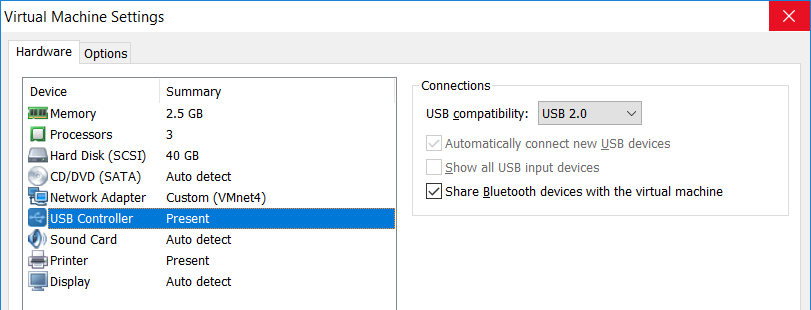
\includegraphics[width=\textwidth]{img/1}}
  \caption{Настройки виртуальной системы}
\end{figure}
После чего, на виртуальной системе будет доступен bluetooth-адаптер.

\section{Выполнение работы}
\subsection{Обзор BlueZ}
\textbf{BlueZ} — стек технологии Bluetooth для Linux. Его цель состоит в том, чтобы сделать реализацию спецификаций стандартов технологии Bluetooth для Linux. Стек BlueZ поддерживает все основные протоколы и уровни Bluetooth. Был первоначально разработан Qualcomm, и доступен для ядра Linux версии 2.4.6 и выше. Во всех, дружественных к пользователю, дистрибутивах Linux, он встроен по умолчанию. На рассматриваемой ОС \textbf{Ubuntu 16.04} в том числе. 

Данный стек покрывает как пространство ядра так и прикладной уровень.
\begin{figure}[H]
  \centering
  \fbox{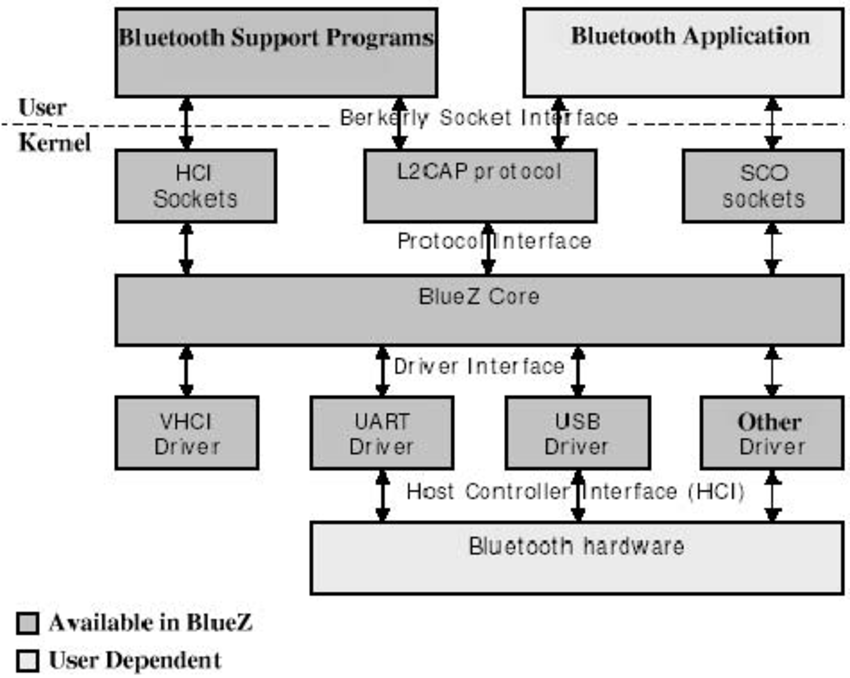
\includegraphics[width=\textwidth]{img/bluez_arch}}
  \caption{Архитектура Bluez}
\end{figure}
В пространстве ядра, уровень \textbf{BlueZ Core} абстрагирует аппаратно-зависимый слой через единый интерфейс.

Bluetooth-адаптер может быть подключен через:
\begin{itemize}
\item \textbf{VHCI} - Virtual Host Controller Interface, имитация реального устройства;
\item \textbf{UART} - Универсальный Асинхронный Приёмопередатчик;
\item \textbf{USB};
\item или как-либо иначе.
\end{itemize}
То есть, как бы устройство не было подключено, интерфейс не изменится.

Интерфейс(\textbf{BlueZ Core}) используется различными протоколами:
\begin{itemize}
\item \textbf{HCI} - хост-контроллер;
\item \textbf{L2CAP} - протокол управления логикой и адаптацией.
\end{itemize}
Стек поставляется со следующими программами:
\begin{itemize}
\item \textbf{bluetoothctl} - программа-интерфейся для работы с bluetooth;
\item \textbf{bluetoothd} - демон bluetooth;
\item \textbf{btmon} - обеспечивает доступ к инфраструктуре монитора подсистемы Bluetooth для чтения трассировки HCI;
\item \textbf{hciconfig} - конфигурация bluetooth-адаптера;
\item \textbf{hcidump} - считывание необработанных данных HCI, поступающих на устройство Bluetooth. Вывод на экран команд, событий и данных в удобочитаемой форме.
\item ...
\end{itemize}
В данной работе будет рассмотрен \textbf{bluetoothctl} - интерфейс bluetooth на прикладном уровне.

\subsection{Обзор bluetoothctl}
Для запуска утилиты, в консоли необходимо ввести \textbf{bluetoothctl}. 
Далее приведено выполнение команд: \textbf{version, help, scan}.
\lstinputlisting[caption=Лог bluetoothctl, language={}]{sourceCode/logs/4.log}
Внимание стоит уделить команде \textbf{scan}, которая была запущена с ключем \textbf{on}, то есть было запущено сканирование.

Далее, на телефоне был включен bluetooth, и в логе появилась запись
\begin{center}
\textbf{[NEW] Device 14:F4:2A:7B:1E:D9 GT-N7100}
\end{center}
То есть сканер, успешно обнаружил мой, личный телефон, вывел его mac-адрес и название устройства.

Для того, чтобы разобраться в функционировании прикладного уровня, предполагается сделать следующие модификации:
\begin{itemize}
\item Изменение версии;
\item При сканировании устройств, автоматическое определение mac-адреса личного телефона, и вывод соответствующего сообщения.
\end{itemize}

\subsection{Модификация прикладного уровня - bluetoothctl}
Был скачан и распакован архив, по следующей ссылке:
\begin{center}
\textbf{http://www.kernel.org/pub/linux/bluetooth/bluez-5.37.tar.xz}
\end{center}
Далее, необходимо понять, где находится отправная точка для модификации. Полный список команд, из предудыщего листинга был выведен не просто-так. Возьмем какую-либо специфичную команду, например - \textbf{set-scan-filter-clear}. Далее применим следующую команду:
\begin{center}
\textbf{sudo grep -rnw '/home/psaer/bluez-5.37' -e 'set-scan-filter-clear'}
\end{center}
Которая рекурсивно ищет среди содержимого файлов нужную строку, в данном случае, выбрануую специфичную команду.
\lstinputlisting[caption=Лог поиска, language={}]{sourceCode/logs/1.log}
Как видно из лога, данную запись содержит файл \textbf{/client/main.c} в строке 1716.

\lstinputlisting[firstnumber=1674,firstline=1674,lastline=1691, caption=.../original/client/main.c]{sourceCode/original/main.c}

Как видно из отрывка кода, в 1674 строке происходит инициализация структуры по обработке cmd команд. Соответственно для каждого названия функции, приведена функция с реализацией.

\subsubsection{Модификация версии}
За вывод версии отвечает функция \textbf{cmd\_version}, откроем её.
\lstinputlisting[firstnumber=1598,firstline=1598,lastline=1601, caption=.../original/client/main.c]{sourceCode/original/main.c}
Как видно из реализации, используется лишь функция \textbf{rl\_printf}. Использование данной функции вместо стандартного \textbf{printf} обусловлено лучшей работой при асинхронных вызовах.

Модифицируем функцию следующим образом:
\lstinputlisting[firstnumber=1603,firstline=1603,lastline=1606, caption=.../modified/client/main.c]{sourceCode/modified/main.c}

\subsubsection{Модификация по определению личного телефона}
Рассмотрим команду \textbf{cmd\_scan}.
\lstinputlisting[firstnumber=880,firstline=880,lastline=903, caption=.../original/client/main.c]{sourceCode/original/main.c}
Как видно из реализации, сперва выполняются различные проверки и подготовки, после чего вызывается функция \textbf{g\_dbus\_proxy\_method\_call}.

Рассмотрим эту функцию.
\lstinputlisting[firstnumber=839,firstline=839,lastline=891, caption=.../original/gdbus/client.c]{sourceCode/original/gdbus/client.c}
В данной реализации, многое завязано на \textbf{d-bus(системе межпроцессного взаимодействия)}. Дальнейший анализ затруден, так как из кода ясно с какими компонентами происходит дальнейшие взаимодействия, поэтому продолжим анализ не заглядывая так глубоко.

При вызове функции \textbf{g\_dbus\_proxy\_method\_call}, одним из её аргуменов является функция - \textbf{start\_discovery\_reply}
\lstinputlisting[firstnumber=863,firstline=863,lastline=878, caption=.../original/client/main.c]{sourceCode/original/main.c}
Исходя из реализации, функция ожидает успешного или не успешного \textbf{discovery} - действия означающего успешный запуск сканирования.

На этом весь прямой поиск заканчивается, более никаких функций, вызывающих интерес не найдено, поэтому применим обратный поиск. Найдем функцию, отвечающую за вывод нового найденного устройства.

Данной функцией оказалась - \textbf{print\_device} из файла \textbf{/client/main.c}.
\lstinputlisting[firstnumber=133,firstline=133,lastline=153, caption=.../original/client/main.c]{sourceCode/original/main.c}
Как видно из реализации, происходит межпроцессное взаимодействие, в ходе которого идет идентификация устройства: получения его адреса, и названия.

Данную функцию вызывает функция \textbf{proxy\_added} из файла \textbf{/client/main.c}.

\lstinputlisting[firstnumber=324,firstline=324,lastline=361, caption=.../original/client/main.c]{sourceCode/original/main.c}
Как видно из реализации, происходит сравнение интерфейсов, далее либо вывод информации в коносль или дополнительные обработки нового устройства.

Теперь узнаем где используется функция \textbf{proxy\_added}.
\lstinputlisting[firstnumber=2059,firstline=2059,lastline=2060, caption=.../original/client/main.c]{sourceCode/original/main.c}
Как видно, данная функция используется в функции \textbf{g\_dbus\_client\_set\_proxy\_handlers} по межпроцессному взаимодействию. То есть, при инициализации программы, на уровне межпроцессного взаимодействия инициализируется обработчик нового устройства.

Для модификации, достаточно изменить функцию \textbf{print\_device}.
\lstinputlisting[firstnumber=134,firstline=134,lastline=158, caption=.../modified/client/main.c]{sourceCode/modified/main.c}
Также, в этот же файл было добавлено подключение \textbf{\#include <string.h>}.
\lstinputlisting[firstnumber=36,firstline=36,lastline=36, caption=.../modified/client/main.c]{sourceCode/modified/main.c}
С помощью функции \textbf{strcmp} происходит сравнение адреса найденного устройства, с предварительно заданным устройством(адресом телефона). И в случае совпадения адресов, выводится соответствующее сообщение.

\subsection{Сборка модифицированного прикладного уровня}
Перед сборкой, необходимо установить следующие зависимости:
\lstinputlisting[caption=Зависимости, language={}]{sourceCode/logs/2.log}
Далее, с помощью команд \textbf{./configure, make, make install} происходит конфигурация, сборка и установка. Логи приложены.


\subsection{Тестирование}
\lstinputlisting[caption=Лог bluetoothctl, language={}]{sourceCode/logs/5.log}
Как видно из лога:
\begin{itemize}
\item текст версии утилиты изменился;
\item при включении bluetooth на телефоне, вывелось соответствующее сообщение.
\end{itemize}


\clearpage
\addcontentsline{toc}{section}{Вывод}
\section*{Вывод}
В данной работе была рассмотрена структура драйвера bluetooth. Был рассмотрен прикладной слой, а также произведены модификации кода, с последующим тестированием.

В отличии от драйвера символьного устройства, в данном случае, на мой взгляд, поддержка драйвера является более сложной задачей, в частности из-за отсутствия документации или каких-либо комментариев в коде. С чем я и столкнулся в данной работе(межпроцессное взаимодействие). В таком случае, для понимания функционирования, необходима отладка и много времени.

В целом, архитектура \textbf{BlueZ} является универсальной, то-есть прикладной интерфейс останется не изменнным, при различных подключениях bluetooth-адаптера.

%------------------------------------------------------------------------------

\nocite{BlueZ1}
\nocite{BlueZ2}
\nocite{BlueZ3}
\nocite{Bluetooth}

\clearpage
\addcontentsline{toc}{section}{Список литературы}
\bibliography{thesis}
\bibliographystyle{ugost2008}

%\clearpage
%\addcontentsline{toc}{section}{Приложения}
%\setcounter{section}{0}
%\section*{Приложение 1} \label{p1:1}
%\textbf{Исходный код драйвера символьного устройства chardev.c}
%\lstinputlisting[caption=chardev.c]{sourceCode/chardev.c}
%
%\section*{Приложение 2} \label{p2:1}
%\textbf{Makefile}
%\lstinputlisting[caption=Makefile]{sourceCode/Makefile}
%
%\section*{Приложение 3} \label{p3:1}
%\textbf{Пользовательская программа для работы с символьным устройством}
%\lstinputlisting[caption=userdev.c]{sourceCode/userdev.c}




\end{document}